\documentclass[11pt]{amsart}
\usepackage[a4paper,margin=1in]{geometry}
\usepackage{amssymb}
\usepackage{tikz}
\usepackage[font=small,labelfont=bf]{caption}
\usepackage[hidelinks]{hyperref}

\colorlet{copper}{orange!75!black}
\colorlet{inkmuted}{black!60}
\tikzset{thin/.style={line width=0.4pt}}

\newtheorem{theorem}{Theorem}
\newtheorem{lemma}[theorem]{Lemma}
\theoremstyle{remark}
\newtheorem{remark}[theorem]{Remark}

\title{Colour the Points, Not the Plane}
\author{Vamshi Jandhyala}
\address{London, United Kingdom}
\email{vamshi.jandhyala@gmail.com}

\begin{document}

\begin{abstract}
If $N$ points in the plane are pairwise at least $1$ apart, at least $N/7$ of them are pairwise more than $\sqrt3$ apart. The known proof colours the points greedily. A tiling proof would instead fix the colouring in advance: cells that cannot hold two of the points, coloured so that cells of one colour are far apart. We show that every such scheme needs at least $(1+\sqrt3)^2\approx7.46$ colours, so no tiling proves $N/7$, and that nine colours of half-open hexagons do work, giving $N/9$. Whether eight colours suffice is open. A seven-colour hexagon argument posted in 2023 fails, and we give two points that break it.
\end{abstract}

\maketitle

\section{The question}

Scatter $N$ points in the plane, pairwise at least $1$ apart. Marconius asked on Mathematics Stack Exchange in July 2015~\cite{MSEa} to show that one can keep at least $N/7$ of them so that the survivors are more than $\sqrt3$ apart. Batominovski answered the same day by colouring the points (Section~\ref{sec:points}). A few days later Pedro asked~\cite{MSEb} for a different proof: tile the plane, colour the tiles, and use the pigeonhole principle. Each tile holds at most one point, tiles of one colour are far apart, so the most popular colour carries at least $N/7$ well-separated points. The asker had triangles or hexagons in mind. That question has no answer.

Before reading on, try to find such a tiling with seven colours. Half-open squares of side $\frac12$ cannot hold two of the points; how many colours do they need?

Formally, a \emph{tiling scheme with $k$ colours} is a partition of the plane into measurable cells, none containing two points at distance $1$ or more, with each cell given one of $k$ colours so that two points in different cells of the same colour are always more than $\sqrt3$ apart. Then each cell holds at most one of the points, and the pigeonhole principle gives $N/k$ survivors. Only two consequences are used below: each cell has diameter at most $1$, and cells of one colour are at least $\sqrt3$ apart.

\begin{theorem}\label{thm:tiling}
Every tiling scheme uses at least $(1+\sqrt3)^2=4+2\sqrt3\approx7.46$ colours, so at least eight.
\end{theorem}

\begin{theorem}\label{thm:nine}
Regular hexagons of side $\frac12$, each owning part of its boundary, coloured by the nine cosets of three times their lattice, form a tiling scheme with nine colours. So a tiling proves the bound $N/9$.
\end{theorem}

The answer to Pedro's question is therefore no for seven colours, yes for nine, and open for eight. Section~\ref{sec:hex} shows where the seven-colour hexagon argument of 2023~\cite{Rosie} goes wrong.

\section{Colouring the points}\label{sec:points}

This section retells Batominovski's proof~\cite{Bato}, because the contrast with a tiling is the point. Join two of the points when they are at most $\sqrt3$ apart; a set with no edges is a set of survivors.

\begin{lemma}\label{lem:thirty}
If $1\le|PQ_1|,|PQ_2|\le\sqrt3$ and $\angle Q_1PQ_2\le30^\circ$, then $|Q_1Q_2|\le1$, with strict inequality when the angle is less than $30^\circ$.
\end{lemma}

\begin{proof}
With $r_i=|PQ_i|$, the cosine rule gives $|Q_1Q_2|^2\le r_1^2+r_2^2-\sqrt3\,r_1r_2$. This is convex in each $r_i$ separately, so on the square $[1,\sqrt3]^2$ it is largest at a corner, and the corner values are $2-\sqrt3$, $1$, $1$ and $6-3\sqrt3$. For an angle below $30^\circ$ the first step is strict.
\end{proof}

\begin{theorem}[Batominovski]\label{thm:seven}
The points can be coloured with seven colours so that points at most $\sqrt3$ apart get different colours. Hence some $N/7$ of them are pairwise more than $\sqrt3$ apart.
\end{theorem}

\begin{proof}
Let $P$ be the lowest point (the leftmost of the lowest, if there is a tie). Its neighbours lie at distances in $[1,\sqrt3]$, in directions from $P$ between $0^\circ$ and $180^\circ$, excluding $180^\circ$. They are pairwise at least $1$ apart, so by Lemma~\ref{lem:thirty} their directions differ by at least $30^\circ$: there are at most six. Colour the other points by induction, and give $P$ a colour its neighbours do not use.
\end{proof}

\begin{figure}[ht]
\centering
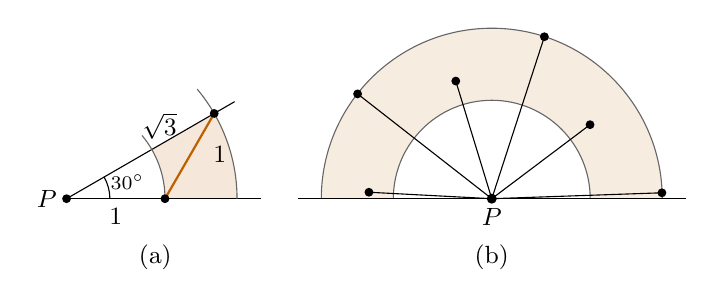
\begin{tikzpicture}
  \begin{scope}
\fill[copper!15] (0:1.250) arc (0:30:1.250) -- (30:2.165) arc (30:0:2.165) -- cycle;
\draw[thin] (0,0) -- (0:2.465); \draw[thin] (0,0) -- (30:2.465);
\draw[inkmuted] (0:1.250) arc (0:40:1.250); \draw[inkmuted] (0:2.165) arc (0:40:2.165);
\draw[thick, copper] (0:1.250) -- (30:2.165);
\fill (0,0) circle (1.6pt) node[left, font=\small] {$P$};
\fill (0:1.250) circle (1.6pt); \fill (30:2.165) circle (1.6pt);
\node[font=\small] at (16:2.025) {$1$};
\draw (0:0.55) arc (0:30:0.55); \node[font=\scriptsize] at (15:0.8) {$30^\circ$};
\node[below, font=\small] at (0:0.625) {$1$}; \node[font=\small] at (38:1.500) {$\sqrt3$};
\node[font=\small] at (1.125,-0.75) {(a)};
\end{scope}
\begin{scope}[shift={(5.4,0)}]
\fill[copper!12] (0:1.250) arc (0:180:1.250) -- (180:2.165) arc (180:0:2.165) -- cycle;
\draw[inkmuted] (0:1.250) arc (0:180:1.250); \draw[inkmuted] (0:2.165) arc (0:180:2.165);
\draw[thin] (-2.465,0) -- (2.465,0);
\draw[thin] (0,0) -- (2.161,0.075); \fill (2.161,0.075) circle (1.6pt);
\draw[thin] (0,0) -- (1.248,0.940); \fill (1.248,0.940) circle (1.6pt);
\draw[thin] (0,0) -- (0.668,2.057); \fill (0.668,2.057) circle (1.6pt);
\draw[thin] (0,0) -- (-0.457,1.494); \fill (-0.457,1.494) circle (1.6pt);
\draw[thin] (0,0) -- (-1.704,1.331); \fill (-1.704,1.331) circle (1.6pt);
\draw[thin] (0,0) -- (-1.560,0.082); \fill (-1.560,0.082) circle (1.6pt);
\fill (0,0) circle (1.8pt) node[below, font=\small] {$P$};
\node[font=\small] at (0,-0.75) {(b)};
\end{scope}

\end{tikzpicture}
\caption{(a) The extreme case of Lemma~\ref{lem:thirty}: points at distances $1$ and $\sqrt3$ from $P$, $30^\circ$ apart, are exactly $1$ apart. (b) The lowest point $P$ and its neighbours in the upper half-annulus, directions at least $30^\circ$ apart, so at most six.}
\label{fig:proof}
\end{figure}

The colouring is chosen after the points are known. That is what a tiling gives up.

\section{Why seven colours cannot tile}

\begin{proof}[Proof of Theorem~\ref{thm:tiling}]
Fix one colour and thicken each of its cells $C$ by the open disc $D$ of radius $\sqrt3/2$. Cells of that colour are at least $\sqrt3$ apart, so the thickened cells $C+D$ are disjoint. The Brunn--Minkowski inequality~\cite{Gardner} gives
\[
\operatorname{area}(C+D)\ \ge\ \Bigl(\sqrt{\operatorname{area}(C)}+\sqrt{\operatorname{area}(D)}\Bigr)^2=\Bigl(\sqrt{A}+\tfrac{\sqrt{3\pi}}2\Bigr)^2,\qquad A=\operatorname{area}(C).
\]
By the isodiametric inequality~\cite{Gardner}, a set of diameter at most $1$ has $A\le\pi/4$, the area of a disc of diameter $1$. The ratio $A/(\sqrt A+c)^2$ increases with $A$, so each cell fills at most
\[
\frac{\pi/4}{\bigl(\tfrac{\sqrt\pi}2+\tfrac{\sqrt{3\pi}}2\bigr)^2}=\frac1{(1+\sqrt3)^2}\approx0.1340
\]
of its thickened region. Now take a disc $B_R$ of radius $R$. Every cell meeting $B_R$ lies in $B_{R+1}$, and its thickening in $B_{R+2}$. So the cells of one colour cover at most $\operatorname{area}(B_{R+2})/(1+\sqrt3)^2$ of $B_R$, and the $k$ colours cover all of it:
\[
\pi R^2\le\frac{k\,\pi(R+2)^2}{(1+\sqrt3)^2}.
\]
Letting $R\to\infty$ gives $k\ge(1+\sqrt3)^2$.
\end{proof}

Read the middle fraction as the best a single colour can do. Each cell must keep a moat of width $\sqrt3/2$ around it, and even the roundest possible cell, a disc of diameter $1$, then fills only $(\frac12)^2/(\frac12+\frac{\sqrt3}2)^2$ of its moated region. Seven colours would need $1/7\approx0.1429$ each. No shape of cell can help: squares, triangles, hexagons and everything else are covered by the same inequality.

\begin{proof}[Proof of Theorem~\ref{thm:nine}]
Place the hexagon centres on the lattice $L$ spanned by $x=(\frac34,\frac{\sqrt3}4)$ and $y=(0,\frac{\sqrt3}2)$, with vertices in the directions $0^\circ,60^\circ,\dots$. Let each hexagon own its interior, its three open edges with outward normals at $30^\circ$, $90^\circ$, $150^\circ$, and its two vertices at $60^\circ$ and $120^\circ$. Each edge is shared by two hexagons with opposite normals and each vertex by three, so these cells partition the plane. The only pairs of a closed hexagon at distance $1$ are opposite vertices, and a cell owns no opposite pair, so no cell holds two points at distance $1$ or more. Colour by the cosets of $3L$. Two hexagons of one colour have centres differing by a nonzero vector of $3L$. The shortest of these, $\pm3x$, $\pm3y$, $\pm3(x-y)$, have length $\frac{3\sqrt3}2$ and point across edges, so these hexagons face each other along parallel edges at distance $\frac{3\sqrt3}2-2\cdot\frac{\sqrt3}4=\sqrt3$; all other vectors of $3L$ have length at least $\frac92$, which leaves a gap of at least $\frac92-1>\sqrt3$. Of two facing edges, exactly one is owned, so two points in different hexagons of one colour are more than $\sqrt3$ apart.
\end{proof}

\section{The hexagon argument}\label{sec:hex}

In 2023 Rosie F answered the original question~\cite{Rosie} with a tiling: hexagons of side $\frac12$ centred on $L$, coloured in seven classes by the standard pattern in which a hexagon's colour differs from those of its six neighbours and the twelve hexagons beyond them. The colour classes are the cosets of the sublattice spanned by $a=3x-y$ and $b=x+2y$. The answer ends by asserting that two points in different hexagons of the same colour are at least $\sqrt3$ apart. Theorem~\ref{thm:tiling} says no seven-colour scheme can achieve this, and Figure~\ref{fig:hex} shows a witness.

\begin{figure}[ht]
\centering
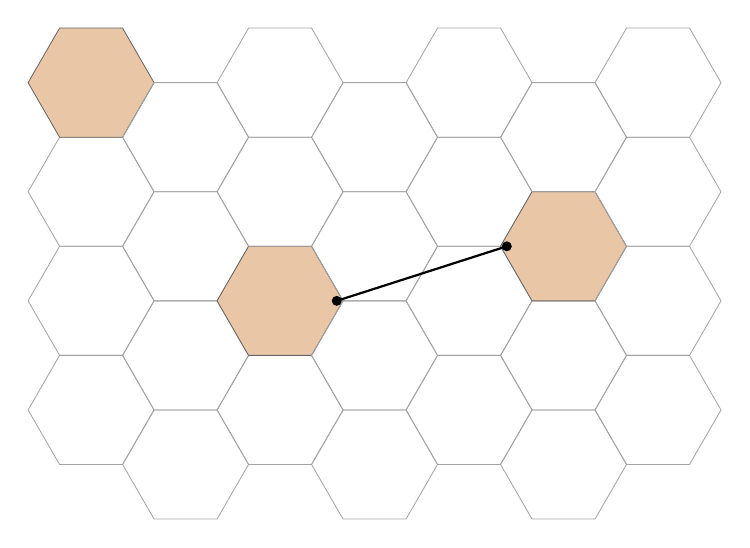
\begin{tikzpicture}
  \draw[inkmuted!60, line width=0.3pt] (-1.600,-1.386) -- (-2.000,-0.693) -- (-2.800,-0.693) -- (-3.200,-1.386) -- (-2.800,-2.078) -- (-2.000,-2.078) -- cycle;
\draw[inkmuted!60, line width=0.3pt] (-1.600,0.000) -- (-2.000,0.693) -- (-2.800,0.693) -- (-3.200,0.000) -- (-2.800,-0.693) -- (-2.000,-0.693) -- cycle;
\draw[inkmuted!60, line width=0.3pt] (-1.600,1.386) -- (-2.000,2.078) -- (-2.800,2.078) -- (-3.200,1.386) -- (-2.800,0.693) -- (-2.000,0.693) -- cycle;
\filldraw[fill=copper!35, draw=inkmuted, line width=0.3pt] (-1.600,2.771) -- (-2.000,3.464) -- (-2.800,3.464) -- (-3.200,2.771) -- (-2.800,2.078) -- (-2.000,2.078) -- cycle;
\draw[inkmuted!60, line width=0.3pt] (-0.400,-2.078) -- (-0.800,-1.386) -- (-1.600,-1.386) -- (-2.000,-2.078) -- (-1.600,-2.771) -- (-0.800,-2.771) -- cycle;
\draw[inkmuted!60, line width=0.3pt] (-0.400,-0.693) -- (-0.800,0.000) -- (-1.600,0.000) -- (-2.000,-0.693) -- (-1.600,-1.386) -- (-0.800,-1.386) -- cycle;
\draw[inkmuted!60, line width=0.3pt] (-0.400,0.693) -- (-0.800,1.386) -- (-1.600,1.386) -- (-2.000,0.693) -- (-1.600,0.000) -- (-0.800,0.000) -- cycle;
\draw[inkmuted!60, line width=0.3pt] (-0.400,2.078) -- (-0.800,2.771) -- (-1.600,2.771) -- (-2.000,2.078) -- (-1.600,1.386) -- (-0.800,1.386) -- cycle;
\draw[inkmuted!60, line width=0.3pt] (0.800,-1.386) -- (0.400,-0.693) -- (-0.400,-0.693) -- (-0.800,-1.386) -- (-0.400,-2.078) -- (0.400,-2.078) -- cycle;
\filldraw[fill=copper!35, draw=inkmuted, line width=0.3pt] (0.800,0.000) -- (0.400,0.693) -- (-0.400,0.693) -- (-0.800,0.000) -- (-0.400,-0.693) -- (0.400,-0.693) -- cycle;
\draw[inkmuted!60, line width=0.3pt] (0.800,1.386) -- (0.400,2.078) -- (-0.400,2.078) -- (-0.800,1.386) -- (-0.400,0.693) -- (0.400,0.693) -- cycle;
\draw[inkmuted!60, line width=0.3pt] (0.800,2.771) -- (0.400,3.464) -- (-0.400,3.464) -- (-0.800,2.771) -- (-0.400,2.078) -- (0.400,2.078) -- cycle;
\draw[inkmuted!60, line width=0.3pt] (2.000,-2.078) -- (1.600,-1.386) -- (0.800,-1.386) -- (0.400,-2.078) -- (0.800,-2.771) -- (1.600,-2.771) -- cycle;
\draw[inkmuted!60, line width=0.3pt] (2.000,-0.693) -- (1.600,0.000) -- (0.800,0.000) -- (0.400,-0.693) -- (0.800,-1.386) -- (1.600,-1.386) -- cycle;
\draw[inkmuted!60, line width=0.3pt] (2.000,0.693) -- (1.600,1.386) -- (0.800,1.386) -- (0.400,0.693) -- (0.800,0.000) -- (1.600,0.000) -- cycle;
\draw[inkmuted!60, line width=0.3pt] (2.000,2.078) -- (1.600,2.771) -- (0.800,2.771) -- (0.400,2.078) -- (0.800,1.386) -- (1.600,1.386) -- cycle;
\draw[inkmuted!60, line width=0.3pt] (3.200,-1.386) -- (2.800,-0.693) -- (2.000,-0.693) -- (1.600,-1.386) -- (2.000,-2.078) -- (2.800,-2.078) -- cycle;
\draw[inkmuted!60, line width=0.3pt] (3.200,0.000) -- (2.800,0.693) -- (2.000,0.693) -- (1.600,0.000) -- (2.000,-0.693) -- (2.800,-0.693) -- cycle;
\draw[inkmuted!60, line width=0.3pt] (3.200,1.386) -- (2.800,2.078) -- (2.000,2.078) -- (1.600,1.386) -- (2.000,0.693) -- (2.800,0.693) -- cycle;
\draw[inkmuted!60, line width=0.3pt] (3.200,2.771) -- (2.800,3.464) -- (2.000,3.464) -- (1.600,2.771) -- (2.000,2.078) -- (2.800,2.078) -- cycle;
\draw[inkmuted!60, line width=0.3pt] (4.400,-2.078) -- (4.000,-1.386) -- (3.200,-1.386) -- (2.800,-2.078) -- (3.200,-2.771) -- (4.000,-2.771) -- cycle;
\draw[inkmuted!60, line width=0.3pt] (4.400,-0.693) -- (4.000,0.000) -- (3.200,0.000) -- (2.800,-0.693) -- (3.200,-1.386) -- (4.000,-1.386) -- cycle;
\filldraw[fill=copper!35, draw=inkmuted, line width=0.3pt] (4.400,0.693) -- (4.000,1.386) -- (3.200,1.386) -- (2.800,0.693) -- (3.200,0.000) -- (4.000,0.000) -- cycle;
\draw[inkmuted!60, line width=0.3pt] (4.400,2.078) -- (4.000,2.771) -- (3.200,2.771) -- (2.800,2.078) -- (3.200,1.386) -- (4.000,1.386) -- cycle;
\draw[inkmuted!60, line width=0.3pt] (5.600,-1.386) -- (5.200,-0.693) -- (4.400,-0.693) -- (4.000,-1.386) -- (4.400,-2.078) -- (5.200,-2.078) -- cycle;
\draw[inkmuted!60, line width=0.3pt] (5.600,0.000) -- (5.200,0.693) -- (4.400,0.693) -- (4.000,0.000) -- (4.400,-0.693) -- (5.200,-0.693) -- cycle;
\draw[inkmuted!60, line width=0.3pt] (5.600,1.386) -- (5.200,2.078) -- (4.400,2.078) -- (4.000,1.386) -- (4.400,0.693) -- (5.200,0.693) -- cycle;
\draw[inkmuted!60, line width=0.3pt] (5.600,2.771) -- (5.200,3.464) -- (4.400,3.464) -- (4.000,2.771) -- (4.400,2.078) -- (5.200,2.078) -- cycle;
\draw[thick] (0.720,0.000) -- (2.880,0.693);
\fill (0.720,0.000) circle (1.8pt);
\fill (2.880,0.693) circle (1.8pt);

\end{tikzpicture}
\caption{The seven-colour hexagon pattern of the 2023 answer, one colour class shaded. The two marked points lie in shaded hexagons and are more than $1$ but only about $1.418$ apart, less than $\sqrt3\approx1.732$.}
\label{fig:hex}
\end{figure}

The points $(0.45,0)$ and $(1.8,\frac{\sqrt3}4)$ lie in the hexagons centred at $0$ and at $a=(\frac94,\frac{\sqrt3}4)$, which have the same colour. Each is $0.45$ from its centre along the horizontal axis, inside the hexagon. Their distance is $\sqrt{1.35^2+\frac3{16}}=\sqrt{2.01}\approx1.418$, more than $1$, so they are a legal pair of points, and less than $\sqrt3$. In fact two hexagons of that class come within $\frac{\sqrt7}2\approx1.323$ of each other.

\section{Verification}

Lemma~\ref{lem:thirty}, the arithmetic of Theorem~\ref{thm:tiling} (the value of the fraction, its monotonicity in $A$, and $1/(1+\sqrt3)^2<1/7$, hence eight colours), and the counterexample of Section~\ref{sec:hex} are proved in Lean~4 with Mathlib~\cite{mathlib}. The Brunn--Minkowski and isodiametric inequalities are quoted~\cite{Gardner}, and Theorem~\ref{thm:seven} is Batominovski's. A Python script checks the lemma on a fine grid, runs the greedy colouring on $300$ random point sets, computes the closest same-coloured hexagons for the seven-class and nine-class patterns, and catches two planted errors (a $40^\circ$ lemma, and the bound $1/(1+\sqrt3)$). Code and Lean files are at~\cite{repo}.

\section*{Acknowledgments}

The problem is Marconius's, the request for a tiling proof is Pedro's, the point-colouring proof is Batominovski's and the hexagon argument is Rosie F's. The analysis, the computations and the Lean formalisation were carried out with Claude Opus~5.5 (Anthropic). The author is responsible for the content.

\begin{thebibliography}{9}
\bibitem{MSEa} Marconius, \emph{Let $S$ be a set of $n$ points in the plane with min spacing of $1$. Prove $S$ has a subset of $\ge n/7$ points with min spacing of $\sqrt{3}$}, Mathematics Stack Exchange question 1378338 (2015), \url{https://math.stackexchange.com/q/1378338}.
\bibitem{Bato} Batominovski, answer to~\cite{MSEa} (2015), \url{https://math.stackexchange.com/a/1378397}.
\bibitem{Rosie} Rosie F, answer to~\cite{MSEa} (2023), \url{https://math.stackexchange.com/a/4680197}.
\bibitem{MSEb} Pedro, \emph{A combinatorial proof by tesselation of the plane}, Mathematics Stack Exchange question 1381502 (2015), \url{https://math.stackexchange.com/q/1381502}.
\bibitem{Gardner} R.~J.~Gardner, \emph{The Brunn--Minkowski inequality}, Bull. Amer. Math. Soc. 39 (2002), 355--405.
\bibitem{mathlib} The mathlib Community, \emph{The Lean mathematical library}, in: Proc. 9th ACM SIGPLAN Int. Conf. on Certified Programs and Proofs (CPP 2020), 367--381.
\bibitem{repo} V.~Jandhyala, code and Lean proofs, \url{https://github.com/jvvk/mathematics/tree/main/colour-the-points}.
\end{thebibliography}

\end{document}
